\chapter{Background}

%\textcolor{red}{As duas proximas secoes devem ser convertidas em um glossario. Inicie esta secao fazendo uma breve apresentacao sobre o pipeline grafico, ate que voce chegue ao conceito de shaders. Depois inclua uma secao explicando o que sao shaders. Depois disso, voce apresentara a secao sobre Vulcan. Note que esta eh uma secao de background para os dois temas centrais do trabalho: shader programming e Vulkan.}

In this chapter, we will introduce the reader to Godot, the tool used to create our application, to GLFW, a supporting library used in our scene visualization window, and to important concepts of computer graphics required for the complete understanding of this thesis. Concepts from linear algebra like vector maths, matrix operations and geometric transformations are presumed to be known.

\section{Godot Engine}
Godot Engine is a 2D and 3D game engine, free and open source under the MIT license. It provides a set of common tools for game development, including many GUI widgets, like buttons, menus, panels and text editors, which is exactly what we needed to build the control window of our application in a way that is very easy to use and to script, while being able to deploy to different platforms. The engine uses its own programming language for scripts, called GDScript, which is similar to Python.

\subsection{GDNative}
GDNative is a module of Godot Engine which adds a new "scripting language" to it \cite{gdnative_post}. In reality, it is not a language, but a precompiled dynamic library that will be loaded into the Godot application. GDNative allows developers to access the Godot API and create scripts using different languages, for example C and C++,  and use these scripts inside Godot as if they were scripts native to the engine.

There are two big use cases for GDNative:

\begin{itemize}
    \item To allow developers to write \textbf{performance critical code} in more efficient languages than GDScript (the scripting language used by Godot Engine). GDScript is a good scripting language, but it was not built for performance. An example task that fits this scenario is generating terrain procedurally;
    \item To allow developers to \textbf{bring third-party code to Godot}. This is useful in game development in general to integrate useful libraries like Steamworks and Google Play Services. In our case, we used it to bring Vulkan code into the application.
\end{itemize}

GDNative is provided as a C API. In order to use other languages, bindings to the original API must be created.

\section{GLFW}
GLFW is an Open Source, multi-platform library for OpenGL, OpenGL ES and Vulkan development on the desktop. It provides a simple API for creating windows, contexts and surfaces, receiving input and events \cite{glfw}.

\section{Graphics pipeline}
In the field of computer graphics, the \textbf{graphics pipeline} is used to generate 2D images out of 3D geometric information in real time applications \cite{shirley_fcg:2002}. Figure \ref{fig:graphics_pipeline} shows a diagram describing the stages of the graphics pipeline. Each stage of the pipeline is responsible for a specific operation; the output of each stage is passed to the next stage to be used as input.

The function performed by each of the stages in the pipeline are described as follows \cite{vulkan_tutorial}:

\begin{itemize}
    \item Input assembler: Collects the raw vertex data from the vertex buffer and may also use an index buffer to repeat certain elements without having to duplicate the vertex data itself;
    \item Vertex shader: Executed for every vertex in the object, generally applies transformations to turn vertex positions from model space to screen space;
    \item Tesselation: Optional stage which subdivides geometry based on certain rules to increase mesh quality;
    \item Geometry shader: Optional stage executed for every primitive (point, line, triangle) which is able to discard or create new primitives;
    \item Rasterization: Breaks down the primitives into fragments, which are the pixel elements that will make up the rendered image. Fragments located outside the screen space are discarded, and vertex data is interpolated across the fragments;
    \item Fragment shader: Invoked for every fragment, determines its color based on the interpolated vertex data outputted by the rasterization stage;
    \item Color blending: Applies operations to mix different fragments that map to the same pixel in the resulting image, usually based upon transparency.
\end{itemize}

\begin{figure}[h]
    \caption{Graphics pipeline}
    \begin{center}
        \includegraphics[width = 7cm]{"vulkan_pipeline"}
    \end{center}
    \label{fig:graphics_pipeline}
    \legend{Source: \cite{vulkan_tutorial}}
\end{figure}

Certain stages can only be controlled by changing their parameters, but the function performed is always the same. These are known as \textit{fixed function stages} and are the ones in green in Figure \ref{fig:graphics_pipeline}.

The other stages, in orange, are known as the \textit{programmable stages}, which means developers can upload source code to the graphics card to apply exactly the operations they intended for that stage.

From the programmable stages, tesselation shaders and geometry shaders are optional, meaning that their functions can be skipped and the pipeline can still work properly. On the other hand, the \textit{vertex shader} and the \textit{fragment shader} are required from the developer and the graphics pipeline cannot function without them.

Shaders always receive data from the previous stage of the pipeline, but they can also define additional parameters to be used in their computations. These parameters are called \textit{uniform variables}. Uniform variables can have their values changed from one draw call to the next, but for every time the shader is executed, the uniform variable will have the exact same value. These variables can be used to, for example, tell the shader where the lights are located in the scene, or provide an image to be used as texture. These values must be supplied from the host application, which manages the graphics pipeline.

The following code represents the basic operation of a vertex shader (in the GLSL language):

\begin{verbatim}
    uniform mat4 modelViewProjection;
    in vec4 position;
    out vec4 clip_position;
    void main() {
        clip_position = modelViewProjection * position;
    }
\end{verbatim}

The first line defines a uniform variable which is a matrix that will transform vertices from local space to clipping space (a normalized space required by the next stages of the pipeline). This matrix accumulates model, view and the projection matrices. The model matrix applies rotation, scale and translation to the object's vertices, transforming them from local space to world space. The view matrix transforms the vertex positions from world space to view space, where the camera is at the origin. Finally, the projection matrix will deform the geometry to apply perspective or orthogonal projections.

The second line describes the vertex attribute that the vertex shader expects to receive from the input assembler. This simple example expects just the vertex position in object space, but it could require other attributes, such as normal vectors or texture coordinates.

The third line describes the output of this shader. Since it is a vertex shader, the vertex position in clip space is required to be an output. Other output variables can be defined, and these variables will be interpolated by the rasterizer and delivered to the fragment shader.

The following code represents the basic operation of a fragment shader:

\begin{verbatim}
    uniform vec4 frag_color;
    out vec4 final_color;
    void main() {
        final_color = frag_color;
    }
\end{verbatim}

The purpose of the fragment shader is to output the color of the fragment. This sample code does just that: a uniform variable is used as color for the fragment. The \texttt{vec4} variable type can be used to represent colors because it holds four floating point values, which are interpreted as red, green, blue and alpha channels.

\section{Graphics APIs}
As we have mentioned, graphics applications require a host application to manage its operation. The means used to do that is through a graphics API. Graphics APIs are a set of routines implemented by graphics cards manufacturers that allow developers to control the hardware. Examples of graphics APIs include Direct3D, OpenGL, Metal and Vulkan. Each API defines their own set of methods and how they are used, and it is up for hardware manufacturers to support the APIs. Some APIs, such as Direct3D and Metal, are proprietary to enterprises (Microsoft and Apple, respectively) and can only be used on their platforms. Others, like OpenGL and Vulkan, are open standards, both provided by the Khronos group, an industry consortium.

Vulkan is a relatively new technology, released version 1.0 in 2016. Since then, several games have been ported to this API, and many game engines have developed rendering backends using Vulkan \cite{vulkan}. This indicates that Vulkan may become the standard graphics API to real-time graphics applications. This work uses the Vulkan API to fulfill a personal goal of creating a functional piece of software using this technology.

\section{Vulkan}
Vulkan is a new generation graphics and compute API that provides high-efficiency, cross-platform access to modern GPUs used in a wide variety of devices from PCs and consoles to mobile phones and embedded platforms \cite{vulkan}.

\subsection{Validation layers}
The Vulkan API is designed around the idea of minimal driver overhead and one of the manifestations of that goal is that there is very limited error checking in the API by default. Even mistakes as simple as setting enumerations to incorrect values or passing null pointers to required parameters are generally not explicitly handled and will simply result in crashes or undefined behavior \cite{vulkan_tutorial}. Vulkan comes with a set of validation and debug layers as part of the Vulkan SDK. When any subset of these layers are enabled they insert themselves automatically into the call-chain of every Vulkan API call issued by the application to perform their job. Validation layers can also report warnings about potential incorrect or dangerous use of the API, and are even capable of reporting performance warnings that allow developers to identify places where the API is used correctly but not used in the most efficient way \cite{vulkan_validation_layers}.

\subsection{Memory management}
While OpenGL drivers manage memory allocations transparently to the programmer, Vulkan not only allows but also requires that programmers allocate device memory (in our case, GPU memory) and bind the memory to the resources used in the application. While this may increase the application's performance if the programmer takes advantage of it, it also requires the programmer to manually manage buffer alignments and aliasing.  The recommended way of allocating memory and creating buffers is described in Figure \ref{fig:vulkan_mem_alloc}.

\begin{figure}[ht]
    \centering
    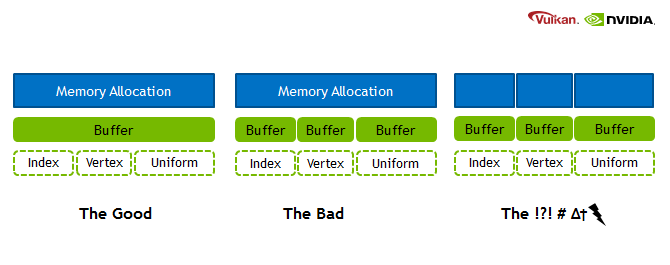
\includegraphics[width = 15cm]{figs/vulkan_memory_strategy.png}
    \caption{Vulkan memory allocation strategies}
    \label{fig:vulkan_mem_alloc}
\end{figure}

This diagram illustrates three memory allocation strategies \cite{vulkan_mem_mgmt}.
The rightmost is the naive approach: for each buffer is performed a "dedicated" memory allocation. This approach is the easiest to implement, since every object allocates, binds and frees their own memory, without taking into account other objects created. It is also the least optimized approach, given that this most likely will not be cache-friendly. It is also important to note that Vulkan devices have a maximum number of memory allocations that can exist simultaneously;
The approach shown in the middle, captioned "The Bad", shows a single memory allocation with various buffers bound to it. This approach is more cache-friendly than the previous one, but it requires the programmer to deal with memory aliasing, offsets and buffer alignments;
The leftmost, captioned as "The Good", is the recommended approach. It represents a single memory allocation bound to a single buffer, with different data loaded to different areas of the buffer. This approach is the most cache-friendly and the most optimized for performance in highly dynamic scenes, but also the most difficult to implement. This setup is possible thanks to Vulkan low-level control of offsets even inside a single buffer, allowing the developer to define "virtual buffers".

In this work, our goal was to build a simple scene with few objects, for the purposes of visualization only. For this reason, we opted to use the naive approach. Implementing a memory management module would not perceivably impact on the performance of the application.

\subsection{Compiling shaders}
Up until OpenGL 4.6, application had to be compile shader source code at run-time, passing a string of high-level source code to the graphics driver. While this allowed the application to run on different hardware, this also forced each GPU manufacturer to provide a GLSL compiler with the device driver, making it difficult for vendors to update and support new versions of the API in their drivers.

\subsubsection{SPIR-V}
The "Standard Portable Intermediate Representation" version "V" (as in "Vulkan") is a binary representation of shader code which device drivers can parse more easily. Application developers, having their shaders written, must compile them into SPIR-V format before loading them in their applications. This contributes for quicker development of device drivers. Support for SPIR-V shaders is included in OpenGL 4.6 and Vulkan 1.0.


% WILL GO TO A "GLOSSARY" OF SORTS
%\section{Rendering}
According to \cite{shirley_fcg:2002}, \emph{rendering} is a term inherited from art and deals with the creation of shaded images from 3D computer models.
%\section{Illumination models}

%\section{Shading models}
%\subsection{Phong shading model}

\section{Shading languages}
Programming languages designed for computer graphics, which are used to define shaders, implementing an illumination model. Various shading languages exist:

\begin{itemize}
    \item CG: \emph{C for Graphics}, developed by NVidia in collaboration with Microsoft, it has been deprecated since 2012;
    \item HLSL: \emph{High-Level Shader Language}, used with DirectX 9 and higher;
    \item GLSL: \emph{OpenGL Shading Language}, used with OpenGL.
\end{itemize}

In this work, all the shader code was written in GLSL. We will not be covering the GLSL language specifics; there are entire books about it, and it goes beyond the scope of this text.

